%===============================================================================
% SYSTEM DESIGN INTERVIEW NOTES
% Live Streaming Platform - SDSE Project
%===============================================================================
% Focus: SOLID Principles, Design Patterns, System Architecture
% Format: Single page, continuous structure, colorful
%===============================================================================

\documentclass[10pt]{article}
\usepackage[utf8]{inputenc}
\usepackage[margin=0.75in]{geometry}
\usepackage{tcolorbox}
\usepackage{tikz}
\usepackage{enumitem}
\usepackage{fancyhdr}
\usepackage{xcolor}
\usepackage{titlesec}
\usepackage{multicol}
\usepackage{amssymb}
\usepackage{enumitem}
\usepackage{tikz}
\usetikzlibrary{shapes,arrows,positioning}

% Color Palette - Modern and Professional
\definecolor{primary}{RGB}{63,94,251}      % Bright Blue
\definecolor{secondary}{RGB}{100,210,255}  % Light Blue
\definecolor{accent}{RGB}{255,101,107}     % Red Accent
\definecolor{success}{RGB}{46,204,113}     % Green
\definecolor{warning}{RGB}{243,156,18}     % Orange
\definecolor{dark}{RGB}{44,62,80}          % Dark Blue-Grey
\definecolor{light}{RGB}{245,247,250}      % Light Grey-Blue
\definecolor{codebg}{RGB}{240,242,245}     % Code Background

% Section Formatting
\titleformat{\section}{
  \vspace{12pt}\large\bfseries\color{primary}
  \titlerule[0.8pt]\vspace{4pt}
}{\thesection}{1em}{}
\titleformat{\subsection}{
  \vspace{8pt}\normalsize\bfseries\color{dark}
}{\thesubsection}{1em}{}
\titleformat{\subsubsection}{
  \vspace{6pt}\normalsize\bfseries\color{secondary}
}{\thesubsection}{1em}{}

% Set compact lists
\setlist[itemize]{leftmargin=*, topsep=3pt, itemsep=3pt}
\setlist[enumerate]{leftmargin=*, topsep=3pt, itemsep=3pt}

% Header/Footer
\pagestyle{fancy}
\fancyhf{}
\fancyhead[L]{\small\color{primary}\textbf{StreamPlatform - SDSE Project}}
\fancyhead[R]{\small\color{primary}\textbf{Interview Notes}}
\fancyfoot[L]{\small\color{dark}\today}
\fancyfoot[C]{}
\fancyfoot[R]{\small\color{dark}\thepage}
\renewcommand{\headrulewidth}{0.5pt}
\renewcommand{\footrulewidth}{0.5pt}

%--------------------------------------------------------------------------------
% DOCUMENT START
%--------------------------------------------------------------------------------
\begin{document}

% Header Box
\noindent
\begin{tcolorbox}[
  colback=primary,
  colframe=primary,
  arc=4pt,
  boxrule=0pt,
 sharp corners,
  before skip=10pt,
  after skip=10pt
]
\begin{minipage}[c]{0.85\textwidth}
  \Huge\bfseries\color{white} Live Streaming Platform
  \normalsize
  \par\medskip
  \large\color{white!90} System Design & Architecture Notes
\end{minipage}%
\begin{minipage}[c]{0.15\textwidth}
\hfill
\includegraphics[width=2.5cm]{placeholder_stream_icon}
\end{minipage}
\end{tcolorbox}

% Tech Stack Stack
\noindent
\begin{tcolorbox}[
  colback=light,
  colframe=primary,
  arc=4pt,
  boxrule=1.5pt,
  sharp corners
]
\begin{center}
\textbf{\large Technology Stack}
\end{center}
\begin{tabular}{@{}llll}
\textbf{Backend:} & NestJS + TypeScript & \textbf{Database:} & PostgreSQL + Prisma ORM \\
\textbf{Frontend:} & React + Vite & \textbf{Streaming:} & Nginx RTMP + HLS \\
\textbf{Real-time:} & Socket.io & \textbf{Auth:} & JWT + Bcrypt \\
\textbf{Testing:} & Jest + Supertest & \textbf{CI/CD:} & GitHub Actions
\end{tabular}
\end{tcolorbox}

%--------------------------------------------------------------------------------
\section*{\color{primary} 1. ARCHITECTURE OVERVIEW}

\noindent
\begin{tcolorbox}[
  colback=white,
  colframe=dark,
  arc=3pt,
  boxrule=1pt,
  before skip=8pt,
  after skip=8pt
]
\textbf{Layered Architecture Pattern:}

\begin{center}
\begin{tikzpicture}[node distance=8pt, auto]
\node (client) [rectangle, draw=primary, fill=primary!10, minimum width=2cm, minimum height=0.6cm] {Client Layer};
\node (api) [rectangle, draw=primary, fill=primary!10, minimum width=2cm, minimum height=0.6cm, below of=client, node distance=1.2cm] {API Layer};
\node (service) [rectangle, draw=primary, fill=primary!10, minimum width=2cm, minimum height=0.6cm, below of=api, node distance=1.2cm] {Service Layer};
\node (repo) [rectangle, draw=primary, fill=primary!10, minimum width=2cm, minimum height=0.6cm, below of=service, node distance=1.2cm] {Repository Layer};
\node (db) [rectangle, draw=success, fill=success!10, minimum width=2cm, minimum height=0.6cm, below of=repo, node distance=1.2cm] {Database};
\node (streaming) [rectangle, draw=accent, fill=accent!10, minimum width=2cm, minimum height=0.6cm, below of=db, node distance=1.2cm] {Streaming Layer};

\draw [->, thick, primary] (client) -- (api);
\draw [->, thick, primary] (api) -- (service);
\draw [->, thick, primary] (service) -- (repo);
\draw [->, thick, success] (repo) -- (db);
\draw [->, thick, accent] (db) -- (streaming);

\node [left=0.3cm of=client, rotate=90, align=center] {\small React + HLS.js};
\node [left=0.3cm of=api, rotate=90, align=center] {\small Controllers};
\node [left=0.3cm of=service, rotate=90, align=center] {\small Business Logic};
\node [left=0.3cm of=repo, rotate=90, align=center] {\small Data Access};
\node [left=0.3cm of=db, rotate=90, align=center] {\small PostgreSQL};
\node [left=0.3cm of=streaming, rotate=90, align=center] {\small Nginx RTMP};
\end{tikzpicture}
\end{center}

\textbf{Key Design Decisions:}
\begin{itemize}
\item \textbf{API-First Design}: All clients (web, mobile) interact via RESTful API
\item \textbf{Separation of Concerns}: Each layer has a single responsibility
\item \textbf{Database Independence}: Prisma ORM abstracts underlying database
\item \textbf{Streaming Isolation}: RTMP/HLS handled separately from core business logic
\end{itemize}
\end{tcolorbox}

%--------------------------------------------------------------------------------
\section*{\color{primary} 2. SOLID PRINCIPLES IN PRACTICE}

\noindent
\begin{tcolorbox}[
  colback=white,
  colframe=dark,
  arc=3pt,
  boxrule=1pt,
  before skip=8pt,
  after skip=8pt
]

\textbf{1. Single Responsibility Principle (SRP)}
\begin{itemize}
\item \textbf{Definition}: A class should have one, and only one, reason to change
\item \textbf{Implementation in Project}:
  \begin{itemize}
  \item \texttt{SubscriptionRepository} - Only handles database operations
  \item \texttt{AuthService} - Only handles authentication logic
  \item \texttt{StreamFactory} - Only handles stream creation
  \end{itemize}
\item \textbf{InterviewTalking Point}: "Each module has a single, well-defined responsibility. If the database schema changes, only the repository changes."
\end{itemize}

\hrule

\textbf{2. Open/Closed Principle (OCP)}
\begin{itemize}
\item \textbf{Definition}: Entities should be open for extension, closed for modification
\item \textbf{Implementation}: \textbf{Strategy Pattern} for viewing plans
\begin{itemize}
\item \texttt{ViewingStrategy} interface defines the contract
\item \texttt{FreeViewingStrategy} - 5 minute limit implementation
\item \texttt{PaidViewingStrategy} - Unlimited implementation
\item Adding new tiers (Student, Enterprise) requires \textbf{no existing code changes}
\end{itemize}
\end{itemize}

\hrule

\textbf{3. Liskov Substitution Principle (LSP)}
\begin{itemize}
\item \textbf{Definition}: Subclasses should be replaceable with their base classes
\item \textbf{Implementation}: \texttt{FreeViewingStrategy} and \texttt{PaidViewingStrategy} both implement \texttt{ViewingStrategy}
\begin{itemize}
\item Both guarantee \texttt{canWatch()} returns \texttt{ViewingResult}
\item The \texttt{ViewerService} works with any strategy without modification
\end{itemize}
\end{itemize}

\hrule

\textbf{4. Interface Segregation Principle (ISP)}
\begin{itemize}
\item \textbf{Definition}: Clients should not depend on interfaces they don't use
\item \textbf{Implementation}: \textbf{ChannelComponent} interface is minimal
\begin{itemize}
\item Only requires \texttt{getDetails()} method
\item \texttt{CommentLeaf} doesn't implement irrelevant methods like \texttt{addStream()}
\end{itemize}
\end{itemize}

\hrule

\textbf{5. Dependency Inversion Principle (DIP)}
\begin{itemize}
\item \textbf{Definition}: High-level modules should not depend on low-level modules
\item \textbf{Implementation}: \textbf{NestJS Dependency Injection}
\begin{itemize}
\item Controllers receive services via constructor injection
\item \texttt{SubscriptionService} receives \texttt{SubscriptionRepository} as interface
\item \texttt{PrismaService} is injected, not instantiated directly
\end{itemize}
\end{itemize}

\end{tcolorbox}

%--------------------------------------------------------------------------------
\section*{\color{primary} 3. DESIGN PATTERNS (Gang of Four)}

\noindent
\begin{tcolorbox}[
  colback=white,
  colframe=dark,
  arc=3pt,
  boxrule=1pt,
  before skip=8pt,
  after skip=8pt
]

\textbf{1. Repository Pattern (Architectural)}
\begin{itemize}
\item \textbf{Purpose}: Decouple data access from business logic
\item \textbf{Problem Solved}: Avoids tight coupling to Prisma/ORM
\item \textbf{Implementation}: \texttt{SubscriptionRepository} extends \texttt{BaseRepository}
\begin{itemize}
\item Defines \texttt{model()} property to specify Prisma model
\item Provides standard CRUD operations automatically
\item Custom methods like \texttt{findByUserId()} for domain-specific queries
\end{itemize}
\item \textbf{Benefit}: Can swap PostgreSQL for MongoDB without changing service code
\end{itemize}

\hrule

\textbf{2. Strategy Pattern (Behavioral)}
\begin{itemize}
\item \textbf{Purpose}: Encapsulate multiple algorithms and make them interchangeable
\item \textbf{Problem Solved}: Eliminates massive if/else chains for different user tiers
\item \textbf{Implementation}: Viewing strategies
\begin{itemize}
\item \texttt{ViewingStrategy} interface with \texttt{canWatch()} and \texttt{getPlanName()}
\item Runtime selection based on user subscription
\item Context: \texttt{SubscriptionService} delegates to injected strategy
\end{itemize}
\item \textbf{Code Location}: \texttt{modules/subscription/strategies/}
\end{itemize}

\hrule

\textbf{3. Composite Pattern (Structural)}
\begin{itemize}
\item \textbf{Purpose}: Treat individual objects and compositions uniformly
\item \textbf{Problem Solved}: Hierarchical data (Channel $\rightarrow$ Streams $\rightarrow$ Comments)
\item \textbf{Implementation}:
\begin{itemize}
\item \texttt{ChannelComponent} interface with \texttt{getDetails()}
\item \texttt{CommentLeaf} - Leaf node (no children)
\item \texttt{StreamComposite} - Node containing comments
\item \texttt{ChannelComposite} - Root node containing streams
\item \texttt{buildChannelComposite()} - Factory to build the tree
\end{itemize}
\item \textbf{Benefit}: Single \texttt{getDetails()} call returns full hierarchy
\end{itemize}

\hrule

\textbf{4. Singleton Pattern (Creational)}
\begin{itemize}
\item \textbf{Purpose}: Ensure single instance of a class
\item \textbf{Implementation}: \texttt{PrismaService}
\begin{itemize}
\item NestJS DI provides single instance across all modules
\item Database connection reused throughout application lifecycle
\item Prevents connection pool exhaustion
\end{itemize}
\end{itemize}

\hrule

\textbf{5. Factory Pattern (Creational)}
\begin{itemize}
\item \textbf{Purpose}: Encapsulate object creation logic
\item \textbf{Implementation}: \texttt{StreamFactory}
\begin{itemize}
\item \texttt{createStandard()} - Standard stream creation
\item \texttt{createLive()} - Immediate Go Live stream
\item \texttt{createScheduled()} - Future scheduled stream
\end{itemize}
\item \textbf{Benefit}: Controllers don't need to know stream construction details
\end{itemize}

\hrule

\textbf{6. Observer Pattern (Behavioral)}
\begin{itemize}
\item \textbf{Purpose}: Notify subscribers of events
\item \textbf{Implementation}: NestJS EventEmitter
\begin{itemize}
\item Events: \texttt{StreamStartedEvent}, \texttt{StreamEndedEvent}
\item Publisher: \texttt{StreamEventEmitter}
\item Listeners: \texttt{StreamEventListener}
\item Modules can subscribe to stream events without tight coupling
\end{itemize}
\end{itemize}

\hrule

\textbf{7. Adapter Pattern (Structural)}
\begin{itemize}
\item \textbf{Purpose}: Convert interface of one class to another
\item \textbf{Implementation}: \texttt{StreamingAdapter}
\begin{itemize}
\item \texttt{IStreamingAdapter} interface defines contract
\item \texttt{NginxRtmpAdapter} implements the interface
\item Unified interface hides RTMP/HLS complexity
\end{itemize}
\item \textbf{Benefit}: Easy to add SRT or WebRTC adapters in future
\end{itemize}

\hrule

\textbf{8. Template Method Pattern (Behavioral)}
\begin{itemize}
\item \textbf{Purpose}: Define algorithm skeleton, allow subclass overrides
\item \textbf{Implementation}: \texttt{BaseService}
\begin{itemize}
\item Defines \texttt{create()}, \texttt{update()} templates
\item Hooks: \texttt{beforeCreate()}, \texttt{afterCreate()}, etc.
\item Subclasses override hooks without changing template flow
\end{itemize}
\end{itemize}

\end{tcolorbox}

%--------------------------------------------------------------------------------
\section*{\color{primary} 4. STREAMING INFRASTRUCTURE}

\noindent
\begin{tcolorbox}[
  colback=white,
  colframe=accent,
  arc=3pt,
  boxrule=1pt,
  before skip=8pt,
  after skip=8pt
]

\textbf{RTMP to HLS Flow:}
\begin{center}
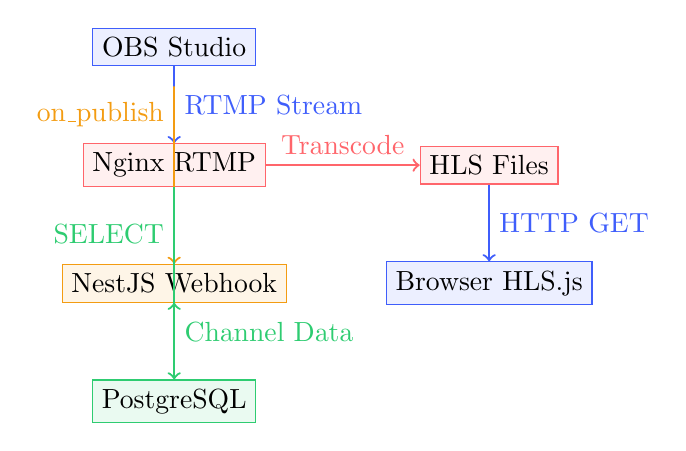
\begin{tikzpicture}[node distance=6pt, auto]
\node (obs) [rectangle, draw=primary, fill=primary!10] {OBS Studio};
\node (rtmp) [rectangle, draw=accent, fill=accent!10, below of=obs, node distance=1.5cm] {Nginx RTMP};
\node (webhook) [rectangle, draw=warning, fill=warning!10, below of=rtmp, node distance=1.5cm] {NestJS Webhook};
\node (db) [rectangle, draw=success, fill=success!10, below of=webhook, node distance=1.5cm] {PostgreSQL};
\node (hls) [rectangle, draw=accent, fill=accent!10, right of=rtmp, node distance=4cm] {HLS Files};
\node (player) [rectangle, draw=primary, fill=primary!10, below of=hls, node distance=1.5cm] {Browser HLS.js};

\draw [->, thick, primary] (obs) -- node {RTMP Stream} (rtmp);
\draw [->, thick, warning] (rtmp) -- node {on\_publish} ++(0,1) -| (webhook);
\draw [->, thick, success] (webhook) -- node {SELECT} ++(0,1) -| (db);
\draw [<-, thick, success] (webhook) -- node {Channel Data} ++(0,-1) -| (rtmp);
\draw [->, thick, accent] (rtmp) -- node {Transcode} (hls);
\draw [->, thick, primary] (hls) -- node {HTTP GET} (player);
\end{tikzpicture}
\end{center}

\textbf{Authentication Flow:}
\begin{enumerate}
\item Broadcaster sends RTMP stream with stream key to Nginx
\item Nginx triggers \texttt{on\_publish} webhook to \texttt{/api/streaming/auth}
\item Backend validates stream key against database
\item HTTP 200 OK allows stream, HTTP 403 blocks it
\item Nginx begins HLS transcoding
\item HLS chunks served via standard HTTP (Port 8080)
\end{enumerate}

\textbf{Why HLS over RTMP?}
\begin{itemize}
\item RTMP requires Flash (deprecated) and special servers
\item HLS works with standard HTTP CDNs (Cloudflare, Vercel)
\item HLS adaptive bitrate for different network conditions
\item Native support in modern browsers
\end{itemize}

\end{tcolorbox}

%--------------------------------------------------------------------------------
\section*{\color{primary} 5. DATABASE SCHEMA (ERD)}

\noindent
\begin{tcolorbox}[
  colback=white,
  colframe=dark,
  arc=3pt,
  boxrule=1pt,
  before skip=8pt,
  after skip=8pt
]

\textbf{Entity-Relationship Diagram:}
\begin{center}
\begin{tikzpicture}[node distance=4pt, every node/.style={font=\scriptsize}]
% User
\node (user) [rectangle, draw=primary, fill=primary!5, minimum width=2cm] {User};
\node (user_attrs) [below of=user, node distance=2pt, align=left] {
id (PK)\\
name\\
email\\
password (bcrypt)\\
createdAt
};

% Subscription (1:1 with User)
\node (sub) [rectangle, draw=warning, fill=warning!5, minimum width=2cm, right of=user, node distance=2.5cm] {Subscription};
\node (sub_attrs) [below of=sub, node distance=2pt, align=left] {
id (PK)\\
plan (FREE/PAID)\\
expiresAt\\
userId (FK)\\
createdAt
};
\draw [thick] (user.east) -- node[above]{1:1} (sub.west);

% Channel (1:1 with User)
\node (channel) [rectangle, draw=accent, fill=accent!5, minimum width=2cm, right of=sub, node distance=2.5cm] {Channel};
\node (channel_attrs) [below of=channel, node distance=2pt, align=left] {
id (PK)\\
name\\
streamKey (unique)\\
userId (FK)\\
createdAt
};
\draw [thick] (user.east) -- ++(0.5,0) |- node[above]{1:1} (channel.west);

% Stream (1:N from Channel)
\node (stream) [rectangle, draw=secondary, fill=secondary!5, minimum width=2cm, below of=channel, node distance=3cm] {Stream};
\node (stream_attrs) [below of=stream, node distance=2pt, align=left] {
id (PK)\\
title\\
status (PENDING/LIVE/ENDED)\\
startedAt\\
endedAt\\
channelId (FK)\\
createdAt
};
\draw [thick] (channel.south) -- ++(0,0.5) -| ++(-2.5,0) |- node[left]{1:N} (stream.north);
\node at ($(channel)!0.5!(stream)$) [rotate=90, below] {1:Many};

% Comment (1:N from Stream)
\node (comment) [rectangle, draw=success, fill=success!5, minimum width=2cm, below of=stream, node distance=2.5cm] {Comment};
\node (comment_attrs) [below of=comment, node distance=2pt, align=left] {
id (PK)\\
content\\
createdAt\\
userId (FK)\\
streamId (FK)
};
\draw [thick] (stream.south) -- ++(0,0.5) -| ++(-2.5,0) |- node[left]{1:N} (comment.north);
\node at ($(stream)!0.5!(comment)$) [rotate=90, below] {1:Many};

\end{tikzpicture}
\end{center}

\textbf{Key Relationships:}
\begin{itemize}
\item \textbf{User $\leftrightarrow$ Subscription}: 1:1 (one subscription per user)
\item \textbf{User $\leftrightarrow$ Channel}: 1:1 (one channel per user)
\item \textbf{Channel $\rightarrow$ Stream}: 1:Many (one channel, many streams)
\item \textbf{Stream $\rightarrow$ Comment}: 1:Many (one stream, many comments)
\end{itemize}

\end{tcolorbox}

%--------------------------------------------------------------------------------
\section*{\color{primary} 6. API ENDPOINTS REFERENCE}

\noindent
\begin{tcolorbox}[
  colback=white,
  colframe=dark,
  arc=3pt,
  boxrule=1pt,
  before skip=8pt,
  after skip=8pt
]

\textbf{Authentication:}
\begin{tabular}{lll}
\textbf{Method} & \textbf{Endpoint} & \textbf{Description} \\
POST & \texttt{/api/auth/register} & Register + create channel \\
POST & \texttt{/api/auth/login} & Login, receive JWT
\end{tabular}

\textbf{Channels:}
\begin{tabular}{lll}
\textbf{Method} & \textbf{Endpoint} & \textbf{Description} \\
GET & \texttt{/api/channels/me} & Get your channel (auth) \\
GET & \texttt{/api/channels/:id} & Get public channel info \\
GET & \texttt{/api/channels/:id/hierarchy} & Full composite tree
\end{tabular}

\textbf{Streams:}
\begin{tabular}{lll}
\textbf{Method} & \textbf{Endpoint} & \textbf{Description} \\
POST & \texttt{/api/streams} & Create stream (auth) \\
PATCH & \texttt{/api/streams/:id/start} & Go live \\
PATCH & \texttt{/api/streams/:id/stop} & End stream \\
GET & \texttt{/api/streams/live} & List live streams \\
GET & \texttt{/api/streams/:id} & Stream details
\end{tabular}

\textbf{Subscriptions:}
\begin{tabular}{lll}
\textbf{Method} & \textbf{Endpoint} & \textbf{Description} \\
POST & \texttt{/api/subscriptions/subscribe} & Upgrade to PAID \\
GET & \texttt{/api/subscriptions/status} & Check plan \\
GET & \texttt{/api/subscriptions/viewing-access} & Get viewing rules
\end{tabular}

\textbf{Streaming:}
\begin{tabular}{lll}
\textbf{Method} & \textbf{Endpoint} & \textbf{Description} \\
GET & \texttt{/api/streaming/urls} & Get RTMP/HLS URLs \\
POST & \texttt{/api/streaming/auth} & Nginx on\_publish webhook
\end{tabular}

\end{tcolorbox}

%--------------------------------------------------------------------------------
\section*{\color{primary} 7. UML DIAGRAMS (Whiteboard Ready)}

\noindent
\begin{tcolorbox}[
  colback=white,
  colframe=dark,
  arc=3pt,
  boxrule=1pt,
  before skip=8pt,
  after skip=8pt
]

\textbf{Class Diagram - Strategy Pattern:}
\begin{center}
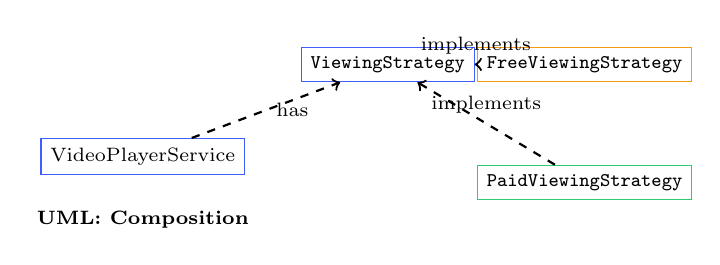
\begin{tikzpicture}[node distance=8pt, every node/.style={font=\scriptsize}]
\node (context) [rectangle, draw=primary, minimum width=2.5cm] {VideoPlayerService};
\node (strategy) [rectangle, draw=primary, minimum width=2cm, above right=1cm of context] {\textbf{\texttt{ViewingStrategy}}};
\node (free) [rectangle, draw=warning, minimum width=2cm, right of=strategy, node distance=2.5cm] {\texttt{FreeViewingStrategy}};
\node (paid) [rectangle, draw=success, minimum width=2cm, below of=free, node distance=1.5cm] {\texttt{PaidViewingStrategy}};

\draw [thick, ->, dashed] (context) -- node[right]{has} (strategy);
\draw [thick, ->, dashed] (free) -- node[above]{implements} (strategy);
\draw [thick, ->, dashed] (paid) -- node[above]{implements} (strategy);
\node [below of=context, node distance=0.8cm] {\textbf{UML: Composition}};
\end{tikzpicture}
\end{center}

\textbf{Class Diagram - Composite Pattern:}
\begin{center}
\begin{tikzpicture}[node distance=8pt, every node/.style={font=\scriptsize}]
\node (comp) [rectangle, draw=primary, minimum width=2cm] {\textbf{\texttt{ChannelComponent}}}};
\node (leaf) [rectangle, draw=success, minimum width=2cm, left=2cm of comp] {\texttt{CommentLeaf}};
\node (stream) [rectangle, draw=warning, minimum width=2cm, right=2cm of comp] {\texttt{StreamComposite}};
\node (channel) [rectangle, draw=accent, minimum width=2cm, above=1.5cm of stream] {\texttt{ChannelComposite}};

\draw [thick, ->] (leaf) -- node[above]{implements} (comp);
\draw [thick, ->] (stream) -- node[above]{implements} (comp);
\draw [thick, ->] (channel) -- node[above]{implements} (comp);
\draw [thick, diamond-, thick] (channel) -- node[above]{contains} (stream);
\draw [thick, diamond-, thick] (stream) -- node[above]{contains} (leaf);
\node [below of=comp, node distance=0.8cm] {\textbf{UML: Aggregation}};
\end{tikzpicture}
\end{center}

\textbf{Sequence Diagram - Stream Authentication:}
\begin{center}
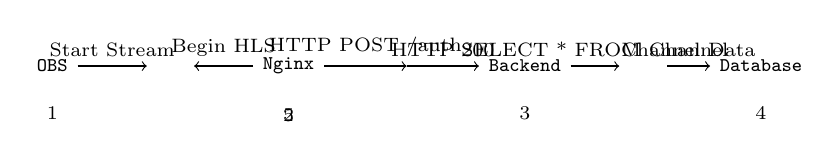
\begin{tikzpicture}[node distance=4pt, every node/.style={font=\scriptsize}]
\node (obs) at (0,0) {\texttt{OBS}};
\node (nginx) at (3,0) {\texttt{Nginx}};
\node (backend) at (6,0) {\texttt{Backend}};
\node (db) at (9,0) {\texttt{Database}};

\draw [->] (obs) -- node[above]{Start Stream} ++(1.2,0);
\draw [->] (nginx) -- node[above]{HTTP POST /auth} ++(1.5,0);
\draw [->] (backend) -- node[above]{SELECT * FROM Channel} ++(1.2,0);
\draw [<-] (db) -- node[above]{Channel Data} ++(-1.2,0);
\draw [<-] (backend) -- node[above]{HTTP 200} ++(-1.5,0);
\draw [->] (nginx) -- node[above]{Begin HLS} ++(-1.2,0);

\node [below=0.2cm of obs] {1};
\node [below=0.2cm of nginx] {2};
\node [below=0.2cm of backend] {3};
\node [below=0.2cm of db] {4};
\node [below=0.2cm of nginx] {5};

\end{tikzpicture}
\end{center}

\end{tcolorbox}

%--------------------------------------------------------------------------------
\section*{\color{primary} 8. INTERVIEW TALKING POINTS}

\noindent
\begin{tcolorbox}[
  colback=white,
  colframe=primary,
  arc=3pt,
  boxrule=1pt,
  before skip=8pt,
  after skip=8pt
]

\textbf{Architecture:}
\begin{itemize}
\item "I used a layered architecture with clear separation: Controllers handle HTTP, Services contain business logic, Repositories manage data access"
\item "The streaming infrastructure is isolated in its own module, using Nginx RTMP for ingestion and HLS for delivery"
\item "All database access goes through Prisma ORM, which provides type safety and makes migrations safe"
\end{itemize}

\textbf{Design Patterns:}
\begin{itemize}
\item "For viewing tiers, I used the Strategy pattern. The context injects the appropriate strategy at runtime, eliminating conditional logic"
\item "The Composite pattern handles the channel hierarchy naturally. A channel contains streams, which contain comments - all implementing the same interface"
\item "Repository pattern abstracts the database. The service layer doesn't care if it's PostgreSQL or MongoDB tomorrow"
\end{itemize}

\textbf{Scalability:}
\begin{itemize}
\item "HLS is HTTP-based, so it works with any CDN. I could add Cloudflare or Vercel for global edge caching"
\item "The stateless nature of the API means I can scale horizontally with multiple NestJS instances behind a load balancer"
\item "Database connections are pooled via Prisma, and the Singleton pattern ensures efficient connection reuse"
\end{itemize}

\textbf{Security:}
\begin{itemize}
\item "Password hashing uses bcrypt with 12 rounds - industry standard for password storage"
\item "JWT tokens are validated on protected routes using guards. The guard checks both authentication and subscription status"
\item "Stream keys are validated via webhook before allowing ingestion - prevents unauthorized streaming"
\end{itemize}

\end{tcolorbox}

%--------------------------------------------------------------------------------
\section*{\color{primary} 9. SCALING CONSIDERATIONS}

\noindent
\begin{tcolorbox}[
  colback=white,
  colframe=warning,
  arc=3pt,
  boxrule=1pt,
  before skip=8pt,
  after skip=8pt
]

\textbf{Current Architecture Strengths:}
\begin{itemize}
\item \textbf{Stateless API}: NestJS services can be replicated behind load balancer
\item \textbf{Database Connection Pooling}: Prisma manages connection pool efficiently
\item \textbf{HLS Delivery}: Works with any CDN (Cloudflare, Vercel, AWS CloudFront)
\item \textbf{CQRS Separation}: Read (HLS) and write (RTMP) are separated
\end{itemize}

\textbf{Future Scaling Paths:}
\begin{itemize}
\item \textbf{Read Replicas}: Add PostgreSQL read replicas for heavy analytics queries
\item \textbf{Microservices}: Split auth, streaming, and notification services
\item \textbf{Redis Caching}: Cache stream metadata, user subscriptions
\item \textbf{WebRTC for Low Latency}: Add WebRTC as alternative to HLS for sub-2s latency
\item \textbf{Object Storage}: Move HLS files to S3/Cloud Storage for durability
\end{itemize}

\textbf{Database Optimization:}
\begin{itemize}
\item Indexes on \texttt{streamKey}, \texttt{channelId}, \texttt{userId}
\item Composite indexes for common query patterns
\item Connection pooling via Prisma to prevent connection exhaustion
\end{itemize}

\end{tcolorbox}

%--------------------------------------------------------------------------------
\section*{\color{primary} 10. PERFORMANCE OPTIMIZATIONS}

\noindent
\begin{tcolorbox}[
  colback=white,
  colframe=success,
  arc=3pt,
  boxrule=1pt,
  before skip=8pt,
  after skip=8pt
]

\textbf{Backend Optimizations:}
\begin{itemize}
\item \textbf{NestJS CLI}: Ahead-of-time compilation for faster startup
\item \textbf{Prisma Query Optimization}: Select only required fields
\item \textbf{Caching Strategy}: Redis cache for frequently accessed data
\item \textbf{Event Emitter}: Asynchronous event processing for non-critical operations
\item \textbf{Batch Operations}: Use Prisma \texttt{createMany}, \texttt{deleteMany}
\end{itemize}

\textbf{Frontend Optimizations:}
\begin{itemize}
\item \textbf{HLS.js}: Adaptive bitrate switching based on network conditions
\item \textbf{WebSocket Reconnection}: Smart reconnection with exponential backoff
\item \textbf{Code Splitting}: React.lazy for route-based code splitting
\item \textbf{Image Optimization}: Lazy loading for channel thumbnails
\end{itemize}

\textbf{Streaming Optimizations:}
\begin{itemize}
\item \textbf{HLS Segments}: 4-second segments for optimal latency/buffer balance
\item \textbf{Adaptive Bitrate}: Multiple quality levels (240p, 360p, 720p, 1080p)
\item \textbf{CDN Caching}: Long cache TTL for static HLS manifests
\end{itemize}

\end{tcolorbox}

%--------------------------------------------------------------------------------
\section*{\color{primary} 11. TESTING STRATEGY}

\noindent
\begin{tcolorbox}[
  colback=white,
  colframe=dark,
  arc=3pt,
  boxrule=1pt,
  before skip=8pt,
  after skip=8pt
]

\textbf{Unit Tests:}
\begin{itemize}
\item \textbf{Repository}: Mock Prisma, test CRUD operations
\item \textbf{Services}: Mock repositories, test business logic
\item \textbf{Strategies}: Test different viewing plans in isolation
\item \textbf{Factories}: Test stream creation logic
\end{itemize}

\textbf{Integration Tests:}
\begin{itemize}
\item \textbf{E2E Tests}: Supertest for API endpoints
\item \textbf{Database Tests}: Test with real PostgreSQL
\item \textbf{WebSocket Tests}: Socket.io client-server interaction
\end{itemize}

\textbf{Test Coverage Areas:}
\begin{itemize}
\item Authentication flows (register, login, JWT validation)
\item Subscription logic (free vs paid tier)
\item Stream lifecycle (create, start, stop, end)
\item Comment system (create, list, hierarchy)
\item Streaming auth webhook
\end{itemize}

\end{tcolorbox}

%--------------------------------------------------------------------------------
\begin{center}
\color{primary}
\Large\bfseries
THE END
\end{center}

\vspace{8pt}

\noindent
\begin{tcolorbox}[
  colback=light,
  colframe=primary,
  arc=3pt,
  boxrule=1pt,
  before skip=8pt,
  after skip=8pt
]
\small
\textbf{Quick Reference - File Locations:}

\begin{tabular}{ll}
Strategy Patterns & \texttt{server/src/modules/subscription/strategies/} \\
Composite Pattern & \texttt{server/src/modules/channel/channel.composite.ts} \\
Factory Pattern & \texttt{server/src/modules/stream/stream.factory.ts} \\
Observer Pattern & \texttt{server/src/modules/stream/stream.observer.ts} \\
Repository Pattern & \texttt{server/src/common/base/base.repository.ts} \\
Template Method & \texttt{server/src/common/base/base.service.ts} \\
Adapter Pattern & \texttt{server/src/modules/streaming/streaming.adapter.ts} \\
Singleton & \texttt{server/src/common/database/prisma.service.ts} \\
Database Schema & \texttt{server/prisma/schema.prisma} \\
\end{tabular}
\end{tcolorbox}

\end{document}
